\documentclass[a4paper]{article}
\usepackage[utf8]{inputenc}
\usepackage{physics}
\usepackage{amsfonts}
\usepackage{amsmath}
\usepackage{float}
\usepackage{graphicx}

\author{Mikael B. Kiste}
\title{FYS3410 - Module II}

\begin{document}
\maketitle

\begin{section}*2
We are presented with the situation of a one-dimensional system of atoms. We would like to know the density of states while using periodic boundary conditions. Let N be the number of atoms in such that atom number 0 and N is the same with the periodic boundary conditions. The distance between each atom is $a$ so the total length of the chain of atoms becomes $L=Na$.
	\begin{subsection}*{a)}
		We describe the phonons by letting the atoms vibrate similarly to a plane wave. The displacement of atom $s$ is described as 
		$$ U_s = U_0 e^{ikas-i\omega t} $$
		Using now the periodic boundary conditions we can get a quantization of the wavenumber
		\begin{align*}
			U_s = U_{s+N}\\
			U_0e^{ikas}e^{-i\omega t} = U_0e^{ika(s+N)}e^{-i\omega t}\\
			e^{ikas} = e^{ikas}e^{ikaN}\\
			e^{ikaN} = 1
		\end{align*}
		This is only true when
		\begin{align*}
			kaN=2 \pi n,\qquad n\in \mathbb{Z}\\
			k = \frac{2\pi n}{Na}
		\end{align*}
		There is a physical restriction on the $n$'s. From the relation between wavelength and wavenumber we have
		\begin{align*}
			\lambda = \frac{2\pi}{k}\\
			\lambda = \frac{aN}{n}
		\end{align*}
		For the first mode $n=1$ the wavelength is $L$, then there are $N$ number of modes until $n=N$ and the wavelength becomes $a$. These are the only physically distinct modes we can have as wavelengths outside this region can not be described distinctly without more atoms (in a similar fashion as with Umklapp scattering).
		Since the $k$'s are uniformly distributed with a distance $\frac{2\pi}{Na}$ the DENSITY (number of states pr. distance) becomes
		$$D(k) = \frac{Na}{2\pi} = \frac{L}{2\pi}$$

		\begin{figure}[H]
			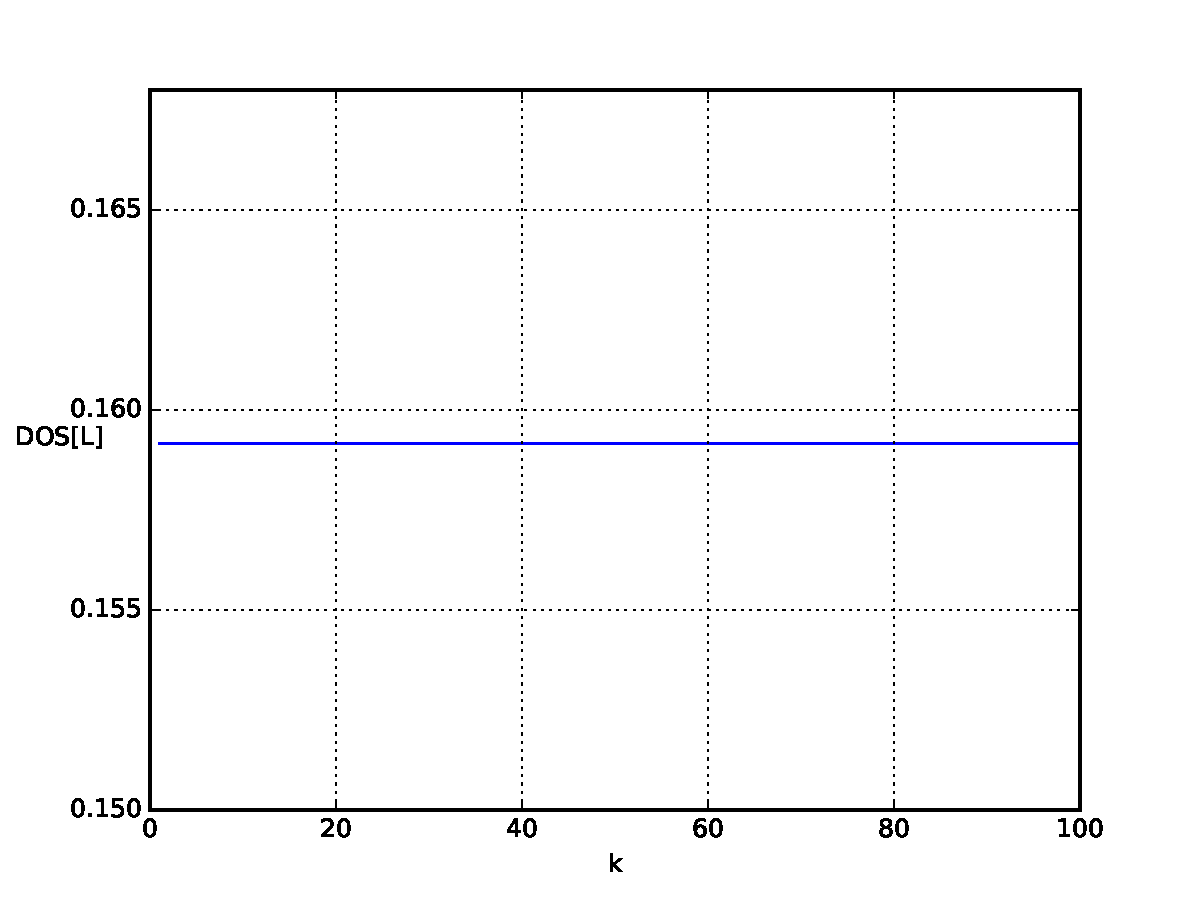
\includegraphics[width = 0.8\linewidth]{2a.pdf}
			\center
		\end{figure}
	\end{subsection}
	\begin{subsection}*{b)}
		If we want the density of states as a function of angular frequency we can use the following relation
		\begin{align*}
			D(\omega)d\omega = D(k)dk\\
			D(\omega)d\omega = \frac{L}{2\pi}\dv{k}{\omega}d\omega\\
			D(\omega)d\omega = \frac{L}{2\pi}v_g^{-1}d\omega\\
		\end{align*}
		We also know that
		$$\omega = \omega_0\sin(ka/2)$$
		This allows us to get an expression for the group velocity but also replace the $k$ with only an $\omega$ dependancy
		\begin{align*}
			k = \frac{2}{a}\sin^{-1}\qty(\frac{\omega}{\omega_0})\\
			v_g = \dv{\omega}{k} \\
			v_g= \dv{k}\omega_0\sin(ka/2)\\
			v_g=\frac{\omega_0a}{2}\cos(ka/2)\\
			v_g=\frac{\omega_0a}{2}\cos(\sin^{-1}\qty(\frac{\omega}{\omega_0}))\\
			v_g = \frac{\omega_0a}{2}\sqrt{1-\qty(\frac{\omega}{\omega_0})^2}
		\end{align*}
		So the density of states becomes
		\begin{align*}
			D(\omega)d\omega = \frac{L}{ \pi\omega_0a\sqrt{1-\qty(\frac{\omega}{\omega_0})^2} } d\omega\\
			D(\omega)d\omega = \frac{N}{ \pi\sqrt{\omega_0^2-\omega^2} } d\omega
		\end{align*}
		\begin{figure}[H]
			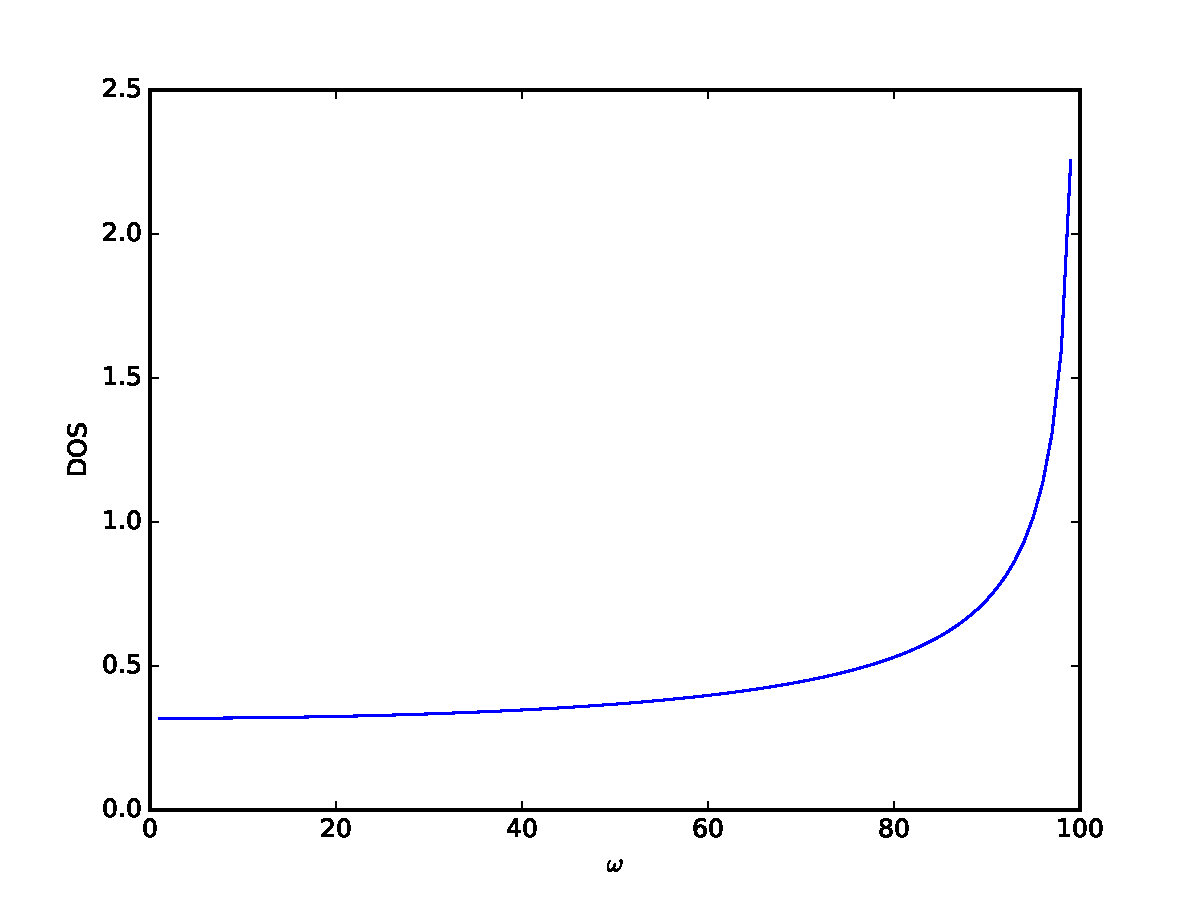
\includegraphics[width = 0.8\linewidth]{2b.pdf}
			\center
		\end{figure}
	\end{subsection}
	\begin{subsection}*{c)}
		The expressions for the density of states in the previous tasks shows that the $k$ dependancy of DOS is a lot simpler than the $\omega$ dependancy. This is quite a common situation and pertains to the boundary conditions directly affecting the wavenumber. In our particular case $D(k)$ is linear while $D(\omega)$ has a more exponential shape.
	\end{subsection}
\end{section}

\begin{section}*3
	Models relating heat capacity to temperature.
	\begin{subsection}*{Debye model}
		The Debye model estimates the phonons contribution to the heat capacity by treating them as in a box (restricted to the crystals dimensions). It is approximately obeyed by most solids at temperatures above room temperature.
		In the graph below is the predicted heat capacity as a function of temperature in the Debye model.
		\begin{figure}[H]
			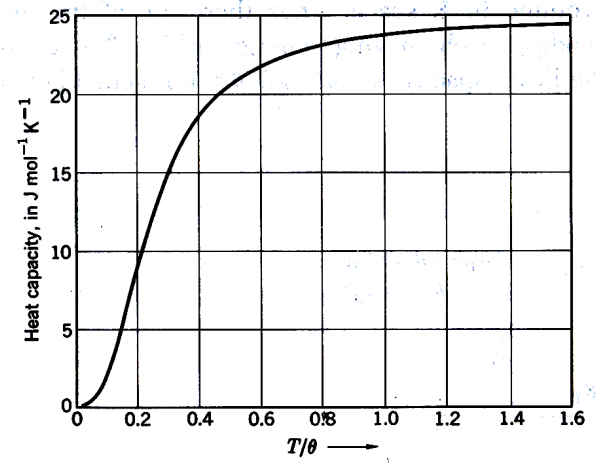
\includegraphics[width = 0.8\linewidth]{debye_graph.png}
			\center
		\end{figure}
		For the smaller temperatures the Debye model predicts a $T^3$ dependancy for the heat capacity which corresponds well to measured trends. The model struggles however at some mid range temperatures, where it is not very accurate.
	\end{subsection}
	\begin{subsection}*{Einstein model}
		In the Einstein model we imagine that each atom is an independent 3D quantum harmoic oscillator. Also, it is assumed that each atom oscillates with the same frequency. Even though this is a somewhat unreasonable assumption as the atoms do not behave completely harmonically, and therefore can not be seen as independent the model still works well at some regions/limits. Especially having a good prediction where the Debye model fails for the intermediate temperatures. As the temperature goes towards zero, however, then the heat capacity falls off too quickly in the Einstein model. This is due to the increasing fraction of phonon energy states awailable at low temperatures that the Einstein model does not take into account. 
	\end{subsection}
	\begin{subsection}*{Dulong-Petit model}
		In this model we assume classical oscillators with continuous energy. At high temperatures it corresponds to the Debye model in the predicted values and shares that models accuracy. However this picture breaks down, of course, at lower temperatures where the quantization has to be taken into account. 
	\end{subsection}

\begin{section}*{4}
	


\end{section}

\begin{section}*6
	The table below show temperature dependencies for heat capacity, $C_V$, phonon mean free path, $\Lambda$, and the thermal conductivity coefficient, $\kappa$. This is in a similar fashion that was discussed in excercise 3.
	\begin{center}
	\begin{tabular}{ | l | l | l | l | }
		\hline
		1 & $C_V$ & $\Lambda$ & $\kappa$ \\ \hline
		Low temperature & $\propto T^3$ & $\Lambda \rightarrow D$ & $\propto T^3$ \\ \hline
		High temperature & $3k_b$ & $\propto T^{-1}$ & $\propto T^{-1}$\\
		\hline
	\end{tabular}
	\end{center}
	Here I have not taken into consideration the Umklapp process that changes the mean free path of the phonons at higher temperatures. In  Umklapp scattering the collision between two phonons as seen in k-space will become a new phonon that is the vector sum of the previous ones. If the new phonon is outside the Brillouin zone it is physically equivalent to some phonon within the Brilloin zone and can be transformed into it by the addition of some reciprocal lattice vector G. In such a process there is a loss of crystal momentum but it is important to note that this is only a pseudomomentum. 
\end{section}

\end{section}







\end{document}